\chapter{线性代数方程组的直接解法}

求解线性代数方程组$Ax=b$:
\begin{equation}
    \begin{bmatrix}
        a_{11}&\cdots&a_{1n}\\
        \vdots&\ddots&\vdots\\
        a_{n1}&\cdots&a_{nn}
    \end{bmatrix}\begin{bmatrix}
        x_1\\\vdots\\x_n
    \end{bmatrix}=\begin{bmatrix}
        b_1\\\vdots\\b_n
    \end{bmatrix}.
\end{equation}
Cramer法则?时间复杂度$\bigo(n\cdot(n+1)!)$

\section{矩阵操作}

\begin{definition}
    {稀疏矩阵}{sparse matrix}
    如果一个矩阵绝大多数元素是0,则称其是稀疏的(sparse)。
\end{definition}

\begin{definition}
    {秩一矩阵}{rank-1 matrix}
    若一个矩阵可以表示成$A=uv\dg$,则其秩为一。
\end{definition}

\begin{theorem}
    {奇异值分解}{singular value}
    根据奇异值分解,可以将矩阵表示成秩一矩阵的线性组合:
    \begin{equation}
        A=U\Sigma V\dg=\sum_i\sigma_iu_iv_i\dg,
    \end{equation}
    其中$U,V$为幺正矩阵。
\end{theorem}

\begin{theorem}
    {矩阵的Hierarchical表示}{Hierarchical matrix}
    考虑分块矩阵
    \[
        A=\begin{bmatrix}
            A_{11}&A_{12}\\
            A_{21}&A_{22}
        \end{bmatrix}
    \]
    $A$一般不是稀疏的,但非对角元$A_{12},A_{22}$是稀疏的,则$Ax$可以分块地写成:
    \[
        Ax=\begin{bmatrix}
            A_{11}&A_{12}\\
            A_{21}&A_{22}
        \end{bmatrix}\begin{bmatrix}
            x_1\\x_2
        \end{bmatrix}=\begin{bmatrix}
            A_{11}x_1+A_{12}x_2\\
            A_{21}x_1+A_{22}x_2
        \end{bmatrix},
    \]
    对$A_{11}x,A_{22}x_2$递归处理。
    \begin{center}
        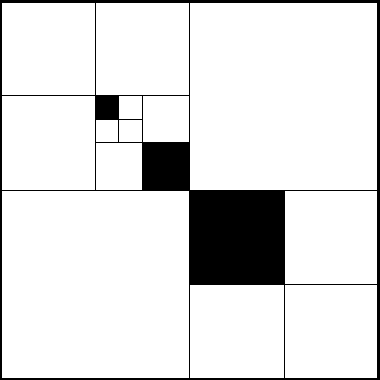
\includegraphics{graphs/Hierarchical.pdf}
        \captionof{figure}{Hierarchical算法示意图,白块表示稀疏部分}
        \label{fig:Hierarchical}
    \end{center}
\end{theorem}

\begin{theorem}
    {矩阵乘法的Strassen算法}{}
    对矩阵乘法$C=AB$分块得:
    \[
        \begin{bmatrix}
            C_{11}&C_{12}\\
            C_{21}&C_{22}
        \end{bmatrix}=\begin{bmatrix}
            A_{11}&A_{12}\\
            A_{21}&A_{22}
        \end{bmatrix}\begin{bmatrix}
            B_{11}&B_{12}\\
            B_{21}&B_{22}
        \end{bmatrix},
    \]
    定义 
    \begin{subequations}
        \begin{align}
            M_1&=(A_{11}+A_{22})(B_{11}+B_{22}),\\
            M_2&=(A_{21}+A_{22})B_{11},\\
            M_3&=A_{11}(B_{12}-B_{22}),\\
            M_4&=A_{22}(B_{21}-B_{11}),\\
            M_5&=(A_{11}+A_{12})B_{22},\\
            M_6&=(A_{21}-A_{11})(B_{11}+B_{12}),\\
            M_7&=(A_{12}-A_{22})(B_{21}+B_{22}),
        \end{align}
    \end{subequations}
    则
    \begin{subequations}
        \begin{align}
            C_{11}&=M_1+M_4-M_5+M_7,\\
            C_{12}&=M_3+M_5,\\
            C_{21}&=M_2+M_4,\\
            C_{22}&=M_1-M_2+M_3+M_6.
        \end{align}
    \end{subequations}
\end{theorem}

\begin{definition}
    {离散Fourier变换}{discrete Fourier transform}
    式\eqref{eqn:Fourier betaj}中定义了一个线性变换,称为离散Fourier变换(discrete Fourier transform, DFT)
    \[
        X_n=\sum_{m=0}^{N-1}x_m\omega^{mn},
    \]
    其中$\omega:=\e{-\i2\pi/N}$是$N$次单位根,对应的变换矩阵为
    \begin{eqnarray}
        F=\begin{bmatrix}
            1&1&1&\cdots&1\\
            1&\omega&\omega^2&\cdots&\omega^{N-1}\\
            1&\omega^2&(\omega^2)^2&\cdots&(\omega^2)^{N-1}\\
            \vdots&\vdots&\vdots&\ddots&\vdots&\\
            1&\omega^{N-1}&(\omega^{N-1})^2&\cdots&(\omega^{N-1})^{N-1}
        \end{bmatrix}
    \end{eqnarray}
    事实上$F$上只有$n$个不同的元素。其逆变换为
    \begin{equation}
        F\iv=\frac1N\bar F.
    \end{equation}
\end{definition}

\begin{theorem}
    {Cooley-Tukey快速Fourier变换}{Cooley-Tukey fast Fourier transform}
    以基2 (radix-2)的情形为例,即$N=2^M$。
    将$X_n$的求和分成偶数项$E_n$和奇数项$O_n$
    \begin{align*}
        X_n&=\sum_{k=0}^{N/2-1}x_{2k}\omega^{2kn}+\sum_{k=0}^{N/2-1}x_{2k+1}\omega^{(2k+1)n}\\
        &=\sum_{k=0}^{N/2-1}x_{2k}\omega^{2kn}+\omega^n\sum_{k=0}^{N/2-1}x_{2k+1}\omega^{2kn}=:E_n+\omega^nO_n,
    \end{align*}
    由于$\omega^N=1$,注意到
    \begin{align*}
        X_{n+N/2}&=\sum_{k=0}^{N/2-1}x_{2k}\omega^{2k(n+N/2)}+\sum_{k=0}^{N/2-1}x_{2k+1}\omega^{(2k+1)(n+N/2)}\\
        &=\sum_{k=0}^{N/2-1}x_{2k}\omega^{2kn}-\omega^n\sum_{k=0}^{N/2-1}x_{2k+1}\omega^{2k}=E_n-\omega^nO_n,
    \end{align*}
    由此便将$N$个$X_n$求和($N^2$)转化成了$N/2$个$E_n,O_n$求和($N^2/2$)。
    采用分而治之的算法思想,可以将DFT的时间复杂度从矩阵向量乘法的$\bigo(N^2)$优化到$\bigo(N\log N)$,这称为快速Fourier变换(fast Fourier transform, FFT)。
    \begin{center}
        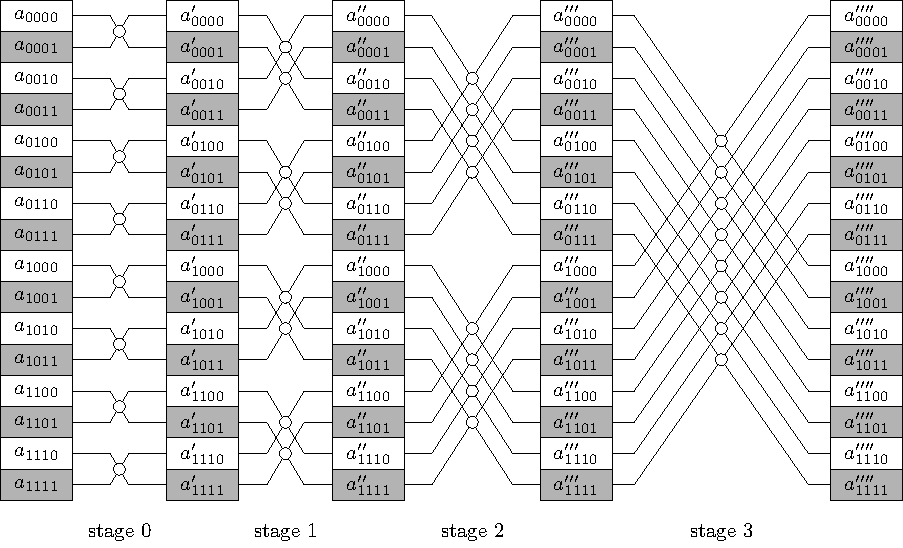
\includegraphics[width=0.8\linewidth]{graphs/FFT.pdf}
        \captionof{figure}{FFT算法示意图($N=2^3=8$)}
        \label{fig:FFT}
    \end{center}
\end{theorem}
\begin{remark}
    对于非基2的情形,$\omega^k$的周期不是基2的,做处理:
    \[
        X_n=\sum_{m=0}^{N-1}x_m\omega^{-mn}=\sum_{m=0}^Nx_m\omega^{[(m-n)^2-m^2-n^2]/2}.
    \]
    定义$\nu_k:=\omega^{k^2/2}$,记$Y_n:=\nu_nX_n,\;z_m:=\nu_m\iv x_m$,则有卷积形式:
    \[
        Y_n=\sum_{m=0}^{N-1}z_m\nu_{m-n}.
    \]
    可以用0将$z_m,\nu_m$延拓,使其周期是一个比$N$大的基2数$N'$。
    再在两端做DFT:
    \begin{align*}
        \sum_{n=0}^{N'-1}Y_n\omega_{N'}^{nk}&=\sum_{n=0}^{N'-1}\sum_{m=0}^{N'-1}z_m\nu_{m-n}\omega_{N'}^{nk}\\
        &=\sum_{m=0}^{N'-1}z_m\omega_{N'}^{mk}\sum_{n=0}^{N'-1}\nu_{m-n}\omega_{N'}^{(n-m)k}=\sum_{m=0}^{N'-1}z_m\omega_{N'}^{mk}\sum_{m=0}^{N'-1}\nu_m\omega_{N'}^{mk}
    \end{align*}
    因此通过对$z_m,\nu_m$做两次DFT、一次向量分量积、一次逆DFT便可得到$Y_n$。 
\end{remark}

\begin{theorem}
    {周期Toeplitz变换}{periodic Toeplitz transform}
    $n$阶矩阵$A$若满足$a_{ij}=c_{i-j}$且序列$c_k$周期为$n$,则$A$称为周期Toeplitz矩阵,且
    \begin{equation}
        A=F\iv\Lambda F,
    \end{equation}
    其中$\Lambda=\diag(\lambda_0,\ldots,\lambda_{n-1})$且
    \begin{equation}
        \lambda_i=\sum_{j=0}^{n-1}c_j\omega^{-ij}.
    \end{equation}
\end{theorem}

\begin{remark}
    $n$阶矩阵$A$若满足$a_{ij}=c_{i-j}$,则该矩阵可以扩展成$2n$阶的周期Toeplitz矩阵。
    \[
        \begin{bmatrix}
            A&*\\ *&*
        \end{bmatrix}
    \]
\end{remark}

\section{Gauss消元法}
\label{sec:Gauss elimination}

\section{稳定性分析}
\label{sec:stability analysis}

在用直接法求解$Ax=b$的过程中,由于舍入误差的存在,必然会导致结果产生误差。因而有必要对可能产生的误差作一估计。
% 通常我们假设在数值处理的过程中计算都是精确的.
\begin{example}
    {数据的微小变化导致解的巨大变化}{}
    方程组
    \[
        \begin{bmatrix}
            10&7&8&7\\
            7&5&6&5\\
            8&6&10&9\\
            7&5&9&10
        \end{bmatrix}\begin{bmatrix}
            x_1\\x_2\\x_3\\x_4
        \end{bmatrix}=\begin{bmatrix}
            32\\23\\33\\31
        \end{bmatrix},\implies\begin{bmatrix}
            x_1\\x_2\\x_3\\x_4
        \end{bmatrix}=\begin{bmatrix}
            1\\1\\1\\1
        \end{bmatrix}.
    \]
    对右端向量做微小的修改
    \[
        \begin{bmatrix}
            10&7&8&7\\
            7&5&6&5\\
            8&6&10&9\\
            7&5&9&10
        \end{bmatrix}\begin{bmatrix}
            x_1'\\x_2'\\x_3'\\x_4'
        \end{bmatrix}=\begin{bmatrix}
            32.1\\22.9\\33.1\\30.9
        \end{bmatrix},\implies\begin{bmatrix}
            x_1'\\x_2'\\x_3'\\x_4'
        \end{bmatrix}=\begin{bmatrix}
            9.2\\-12.6\\4.5\\-1.1
        \end{bmatrix}.
    \]
    对系数矩阵做一微小的修改
    \[
        \begin{bmatrix}
            10&7&8.1&7.2\\
            7.08&5.04&6&5\\
            8&5.98&9.89&9\\
            6.99&4.99&9&9.98
        \end{bmatrix}\begin{bmatrix}
            x_1''\\x_2''\\x_3''\\x_4''
        \end{bmatrix}=\begin{bmatrix}
            32\\23\\33\\31
        \end{bmatrix},\implies\begin{bmatrix}
            x_1''\\x_2''\\x_3''\\x_4''
        \end{bmatrix}=\begin{bmatrix}
            -81\\137\\-34\\22
        \end{bmatrix}.
    \]
\end{example}

\begin{definition}
    {条件数}{condition number}
    给定诱导的矩阵范数$\norm\cdot$,可逆矩阵$A$的条件数(condition number)为
    \begin{equation}
        \cond(A)\equiv\norm A\nnorm{A\iv}.
    \end{equation}
\end{definition}

\begin{theorem}
    {解的扰动定理}{}
    给定可逆矩阵$A$和微小扰动$\D A$,满足
    \[
        \frac{\norm{\D A}}{\norm A}<\frac1{\cond(A)},
    \]
    则$(A+\D A)$也可逆,考察线性方程组$Ax=b$及其扰动解
    \[
        (A+\D A)(x+\D x)=b+\D b,
    \]
    则有
    \begin{equation}
        \frac{\norm{\D x}}{\norm x}\leq\frac{\cond(A)}{1-\norm{A\iv}\norm{\D A}}\biggkh{\frac{\norm{\D A}}{\norm A}+\frac{\norm{\D b}}{\norm b}}.
    \end{equation}
\end{theorem}

\begin{proof}
    由扰动定理\thmref{thm:perturbation theorem II}知$(A+\D A)$可逆且
    \begin{equation}
        \norm{(A+\D A)\iv}\leq\frac{\norm{A\iv}}{1-\norm{A\iv}\norm{\D A}}.
    \end{equation}
    由
    \begin{align*}
        \D x&=(A+\D A)\iv(b+\D b)-x\\
        &=(A+\D A)\iv(b+\D b-(A+\D A)x)\\
        &=(A+\D A)\iv(\D b-\D Ax),
    \end{align*}
    两边取范数
    \begin{align*}
        \norm{\D x}&\leq\norm{(A+\D A)\iv}(\norm{\D b}+\norm{\D A}\norm x)\\
        &\leq\frac{\norm{A\iv}}{1-\norm{A\iv}\norm{\D A}}\biggkh{\frac{\norm{\D A}}{\norm A}\norm A\norm x+\frac{\norm{\D b}}{\norm b}\norm A\norm x}.
        \qedhere
    \end{align*}
\end{proof}

\begin{theorem}
    {矩阵相对奇异性的度量}{}
     
\end{theorem}
